
\section{Convergence rates for the $\mu$-best averaging approach}
\label{sec:mubestrate}
% \begin{lemma} 
% \label{lem:condit-upper} 
% Let $f$ be a function satisfying Assumption~\ref{ass:principal}. Let $h\in[0,\max f]$. Let $\lambda$ and $\mu$ be two integers such that $1\leq \mu \leq \lambda-1$. Then we have
% \[
% \mathbb{E}_{X_{1},...X_{\lambda}\sim U(B(0,r))}\left[f(\bar{X}_{(\mu)})\mid f(X_{(\mu+1)})=h\right]\le C\frac{h}{\mu}+O(h^{\alpha-1})
% \]
% as $h\rightarrow0$, for some $C>0$ independent from $h$, $\mu$ and $\lambda$. \end{lemma} 
In the next section we focus on the case where we average the $\mu$ best samples among the $\lambda$ samples.  We first prove a lemma when the sampling is conditional on the $(\mu+1)$-th value.
\begin{lemma} 
\label{lem:condit-upper} 
Let $f$ be a function satisfying Assumption~\ref{ass:principal}. There exists a constant $C_3>0$ such that for all $h\in[0,\max f]$ and $\lambda$ and $\mu$ two integers such that $1\leq \mu \leq \lambda-1$, we have the following conditional upper bound:
\[
\mathbb{E}_{X_{1},...X_{\lambda}\sim U(B(0,r))}\left[f(\bar{X}_{(\mu)})|f(X_{(\mu+1)})=h\right]\le C_3\left(\frac{h}{\mu}+h^{\alpha-1}\right).
\]


\end{lemma} 
\begin{proof}
We first decompose the expectation as follows.
\begin{align}
\mathbb{E}&_{X_{1},...X_{\lambda}\sim U(B(0,r))}  \left[f(\bar{X}_{(\mu)})|f(X_{(\mu+1)}))=h\right]\nonumber\\
 & =\mathbb{E}_{X_{1},...X_{\mu}\sim U(S_{h})}\left[f(\bar{X}_{\mu})\right]\nonumber\\
 & =\mathbb{E}_{X_{1},\cdots,X_{\mu}\sim U(S_{h})}\left[\lVert \bar{X}_{\mu}-x^\star\rVert_{\mathbf{H}}^2\right]\label{eq:first-term}\\
 &+\mathbb{E}_{X_{1},\cdots,X_{\mu}\sim U(S_{h})}\left[\lVert\bar{X}_{\mu}-x^\star\rVert^{\alpha}_{\mathbf{H}}\varepsilon(\bar{X}_{\mu}-x^\star)\right]\label{eq:snd-term}
\end{align}
where we have use the same argument as in Remark~\ref{rk:samples} in the first equality.
We will treat the terms~\eqref{eq:first-term} and~\eqref{eq:snd-term} independently. We first look at~\eqref{eq:first-term}. We have the following ``bias-variance'' decomposition.
\begin{align*}
\mathbb{E}_{X_{1},\cdots,X_{\mu}\sim U(S_{h})}\lVert\bar{X}_{\mu}-x^{\star}\rVert^{2}_{\mathbf{H}} 
=&(1-\frac{1}{\mu})\lVert\mathbb{E}_{X\sim U(S_{h})}X-x^{\star}\rVert^{2}_{\mathbf{H}}\\
&+\frac{1}{\mu}\mathbb{E}_{X\sim U(S_{h})}\lVert X-x^{\star}\rVert^{2}_{\mathbf{H}}
\end{align*}
We will use Lemma~\ref{lemma:sandwich-set}. We have $A_h\subset S_h\subset B_h$. Hence for the variance term
\[
\frac{1}{\mu}\mathbb{E}_{X\sim U(S_{h})}\lVert X-x^{\star}\rVert^{2}_{\mathbf{H}}\leq\frac{1}{\mu}\mathbb{E}_{X\sim U(S_{h})} \phi_+(h)^{2} \leq \frac{\phi_+(h)^{2}}{\mu}\sim_{0} \frac{h}{\mu}.
\]
where $\sim_0$ means ''is equivalent to $\dots$ when $h\to0$, in other words, $u(h)\sim_0 v(h)$ iff $\frac{u(h)}{v(h)}\to 0$ as $h\to0$. For the bias term, recall that \[\mathbb{E}_{X\sim U(S_{h})}\left[X-x^\star\right] = \frac{1}{\mathrm{vol}(S_h)}\int_{S_h} (x-x^\star) dx.\] We then have by inclusion of sets
\begin{align*}
    \mathrm{vol}(A_h)\leq \mathrm{vol}(S_h)\leq \mathrm{vol}(B_h)
\end{align*}
Note that the volume of the $d$-dimensional ellipsoid $B_h$ satisfies $\mathrm{vol}(B_h)=\phi_+(h)^{d}\frac{\omega_{d}}{\mathrm{det}(\mathbf{H})}$ with $\omega_{d}=\mathrm{vol}(B(0,1))$ and similarly for $A_h$.
From this we deduce by the squeeze theorem that 
\[\mathrm{vol}(S_h)\sim \frac{\omega_dh^{d/2}}{\mathrm{det}(\mathbf{H})}.\]We now decompose the integral 
\begin{align*}
\int_{S_{h}}(x-x^\star)dx & =\int_{A_{h}}(x-x^\star)dx+\int_{S_{h}\setminus A_{h}}(x-x^\star)dx\\
 & =\int_{S_{h}\setminus A_{h}}(x-x^\star)dx
\end{align*}
(because $A_{h}$ is an ellipsoid centered at $x^\star$ hence the integral of $x-x^\star$
over it is $0$). We then upper-bound using the triangle inequality for the $\mathbf{H}-$norm:
\begin{align*}
\lVert\int_{{S}_{h}\setminus A_{h}}(x-x^\star)dx\rVert_{\mathbf{H}} &\leq \int_{{S}_{h}\setminus A_{h}}\lVert x-x^\star\rVert_{\mathbf{H}} dx\\
& \le \phi_+(h)\mathrm{vol}({S}_{h}\setminus A_{h})\\
 & = \phi_+(h)(\mathrm{vol}({S}_{h})-\mathrm{vol}(A_{h}))\\
 &\leq \phi_+(h)(\mathrm{vol}(B_h)-\mathrm{vol}(A_h))\\
 & \sim d\frac{\omega_d}{\mathrm{det}(\mathbf{H})}\frac{m+M}{2}h^{d/2}h^{(\alpha-1)/2}
\end{align*}
For the last equivalent, we used a Taylor expansion for the volume of $A_h$ and $B_h$. We conclude that there exist $h_1>0$ and a constant $C>0$ not depending on $\lambda$ and $\mu$ such that for $h\leq h_1$,
\begin{align*}
\lVert\mathbb{E}_{X\sim U(S_{h})}\left[X\right]-x^\star\rVert^{2}_{\mathbf{H}} \leq C h^{\alpha-1}
\end{align*}
Since $h$ is upper bounded by $\max f$, the previous inequality can be extended to $h\in[0,\max f]$, with a possibly larger constant still not depending on $\lambda$ and $\mu$. Let us now upper bound the remainder term~\eqref{eq:snd-term}.
As $\varepsilon \leq M$ by assumption, we can write
\begin{align*}
\mathbb{E}_{X_{1},\cdots,X_{\mu}\sim U(S_{h})}&\left[\lVert\bar{X}_{\mu}-x^\star\rVert^{\alpha}_{\mathbf{H}}\varepsilon(\bar{X}_{\mu}-x^\star)\right]\\
&\le M\mathbb{E}_{X_{1},\cdots,X_{\mu}\sim U(S_{h})}\left[\lVert\bar{X}_{\mu}-x^\star\rVert^{\alpha}_{\mathbf{H}}\right]
\end{align*}

We have $X_{1},\cdots,X_{\mu}\in S_{h}\subset B_{h}$
hence by the convexity of $B_h$ (which is a ball for the $\mathbf{H}$-norm) we also have $\bar{X}_{\mu}\in B_{h}$ and
thus, for $h$ sufficiently small, we have:
\[
\lVert\bar{X}_{\mu}-x^\star\rVert_{\mathbf{H}}\le \phi_+(h).
\]
Note that $\phi_+(h)\sim_{0} \sqrt{h} $ thus, for $h$ sufficiently small, $ \lVert\bar{X}_{\mu}-x^\star\rVert_{\mathbf{H}}\le 1$
almost surely, hence, as $\alpha > 2$
\begin{align*}
\lVert\bar{X}_{\mu}-x^\star\rVert^{\alpha}_{\mathbf{H}}\leq \lVert\bar{X}_{\mu}-x^\star\rVert^{2}_{\mathbf{H}}
\end{align*}
almost surely. Since $h$ is upper bounded, we have the existence of a constant $C'>0$ not depending on $\lambda$ and $\mu$, such that for all $h\in [0,\max f]$,
\begin{align*}
\lVert\bar{X}_{\mu}-x^\star\rVert^{\alpha}_{\mathbf{H}}\leq C'\lVert\bar{X}_{\mu}-x^\star\rVert^{2}_{\mathbf{H}}
\end{align*}
Thus we can upper bound the remainder with the same bounds as the one for the main term (up to constants), for any $h\in[0,\max f]$.
We now group the ``main'' term and remainder term to get the existence of a constant $C_3>0$ not depending on $\lambda$ and $\mu$ such that for all $h\in [0,\max f]$,
\[
\mathbb{E}_{X_{1},...X_{\lambda}\sim U(B(0,r))}\left[f(\bar{X}_{(\mu)})|f(X_{(\mu+1)})=h\right]\le C_3\left(\frac{h}{\mu}+h^{\alpha-1}\right)\quad.
\]


\end{proof}



% \begin{theorem} 
% Under assumptions~\ref{ass:principal}
% and also with $1\le \mu<n\big(\frac{L(r-||x^{\star}||)^{2}}{r}\big)^{d}$
% we have 
% \begin{align*}
% \mathbb{E}_{X_{1},...X_{\lambda}\simB(0,r)} & \left[f(\bar{X}_{(\mu)})-f(x^{\star})\right]\\
%  & \leq C\bigg[\mu^{\alpha/d}n^{\alpha/d}+\mu^{2/d-1}n^{-2/d}+\mu^{2/d-1}a^{n}+\exp(-\frac{2\varepsilon^{2}}{n})\bigg]
% \end{align*}
% for some $C\ge0$ depending on $L,\mu,r,d,x^{\star}$, some $|a|<1$
% and $\varepsilon=n\big(\frac{L(r-||x^{\star}||)^{2}}{r}\big)^{d}-\mu$.
% With the choice $\mu=C'n^{\frac{\alpha-2}{\alpha+d-2}}$, we get a main
% rate of $n^{-\alpha/(\alpha+d-2)}$ which is \emph{strictly }better
% than the rate of the 1-best whenever $\alpha>2$, $d>2$ 
% \end{theorem} 

We are now set to prove our main result, which is an upper convergence rate for the $\mu$-best approach. This is the main result of the paper.
\begin{thm}\label{thm:principal}
Let $f$ be a function satisfying Assumption~\ref{ass:principal}.  Let $(\mu_\lambda)_{\lambda\in\mathbb{N}}$ be a sequence of integers such that $\forall\lambda\geq 2$, $1\leq \mu_\lambda \leq \lambda -1$ and $\mu_\lambda\to\infty$. Then, there exist two constants $C,C'>0$ and $\Tilde{\lambda}\in \mathbb{N}$ such that  for $\lambda\geq\Tilde{\lambda}$, we have the upper bound: 
\begin{align*}
 \mathbb{E}_{X_{1},\dots,X_{\lambda}\sim U(B(0,r))}\left[f(\bar{X}_{(\mu_\lambda)})\right] \leq C\frac{\mu_\lambda^{\frac{2(\alpha-1)}{d}}}{\lambda^{\frac{2(\alpha-1)}{d}}}+C'\frac{\mu_\lambda^{\frac{2}{d}-1}}{\lambda^{\frac{2}{d}}}\quad.
\end{align*}
In particular if $\mu_{\lambda}\sim C^{''}\lambda^{\frac{2(\alpha-2)}{d+2(\alpha-2)}}$
for some $C^{''}>0$, we obtain:
\begin{align*}
\mathbb{E}_{X_{1},\dots,X_{\lambda}\sim U(B(0,r))}\left[f(\bar{X}_{(\mu_{\lambda})})\right] & \le C^{'''}\lambda^{-\frac{2(\alpha-1)}{d+2(\alpha-2)}}
\end{align*}
for some $C'''>0$ independent of $\lambda$.\end{thm}

{We note that $\frac{\mu}{\lambda}\to 0$ as $\lambda\to 0$. This makes sense intuitively: we average points in a sublevel set, which makes sense only if, asymptotically in $\lambda$, this sublevel set shrinks to a neighborhood of the optimum.}

\begin{proof}
The random variable $f(X_{(\mu_\lambda+1)})$ takes its values in $[0,\max f]$ almost surely. As such, thanks to Lemma~\ref{lem:condit-upper}, there exists a constant $C_3>0$ such that for all $\lambda\geq 1$:
 \begin{align*}
      \mathbb{E}\left[f(\bar{X}_{(\mu_\lambda)})\right]&=\mathbb{E}\left[\mathbb{E}\left[f(\bar{X}_{(\mu_\lambda)})\mid f(X_{(\mu_\lambda+1)}) \right]\right]\\
        &\leq \mathbb{E}\left[C_3\left(\frac{1}{\mu_\lambda}f(X_{(\mu_\lambda+1)})+f(X_{(\mu_\lambda+1)})^{\alpha-1}\right)\right]\\
      &= C_3\left(\frac{1}{\mu_\lambda}\mathbb{E}\left[f(X_{(\mu_\lambda+1)})\right]+\mathbb{E}\left[f(X_{(\mu_\lambda+1)})^{\alpha-1}\right]\right)
 \end{align*}
 
Let us first bound $\mathbb{E}\left[f(X_{(\mu_\lambda+1)})\right]$. Thanks to Lemma~\ref{lem:lower1best}, there exist a constant $C_2>0$ and $\lambda_2\in \mathbb{N}$ such that:
\begin{align*}
  \mathbb{E} \left[f(X_{(\mu_\lambda+1)})\right]&\leq \frac{\mu_\lambda^{2/d}}{C_2}\mathbb{E}\left[\mathbb{E} \left[f(X_{(1)})\mid f(X_{(\mu_\lambda+1)})\right]\right]\\
  &=\frac{\mu_\lambda^{2/d}}{C_2}\mathbb{E} \left[f(X_{(1)})\right]
\end{align*}

Thanks to Lemma~\ref{lem:upper1best}, there exists a constant $C_0>0$ and an integer $\lambda_0\in \mathbb{N}$ such that for all integers $ \lambda\geq \lambda_0$:
$$\mathbb{E}_{X_1,\cdots,X_\lambda\sim U(B(0,r))}\left[ f\left(X_{(1)}\right)\right] \leq C_0 \lambda^{-\frac2d}\quad. $$

Then finally for $\lambda\geq\max(\lambda_0,\lambda_2)$
\begin{align*}
    \mathbb{E} \left[f(X_{(\mu_\lambda+1)})\right]\leq\frac{C_0}{C_2} \frac{\mu_\lambda^{2/d}}{\lambda^{2/d}}\quad.
\end{align*}

For the term $\mathbb{E}\left[f(X_{(\mu_{\lambda}+1)})^{\alpha-1}\right]$,
we write thanks to Lemma~\ref{lem:lower1best}
\[
\mathbb{E}\left[f(X_{(\mu_{\lambda}+1)})^{\alpha-1}\right]\leq\frac{\mu_{\lambda}^{2(\alpha-1)/d}}{C_{2}^{\alpha-1}}\mathbb{E}\left[\mathbb{E}\left[f(X_{(1)})\mid f(X_{(\mu_{\lambda}+1)})\right]^{\alpha-1}\right].
\]
Then, by Jensen's inequality for the conditional expectation, we get
\[
\mathbb{E}\left[f(X_{(\mu_{\lambda}+1)})^{\alpha-1}\right]\le\frac{\mu_{\lambda}^{2(\alpha-1)/d}}{C_{2}^{\alpha-1}}\mathbb{E}\left[f(X_{(1)})^{\alpha-1}\right].
\]
Similarly to Lemma~\ref{lem:upper1best}, by replacing $\lVert X-x^\star\rVert^2$ by $\lVert X-x^\star\rVert^{2(\alpha-1)}$, one can show $\mathbb{E}\left[f(X_{(1)})^{\alpha-1}\right]\le C'_{3}\lambda^{-2(\alpha-1)/d}$
for some $C'_{3}>0$ independent of $\lambda$. We thus get $\mathbb{E}\left[f(X_{(\mu_{\lambda}+1)})^{\alpha-1}\right]\le C\frac{\mu_{\lambda}^{2(\alpha-1)/d}}{\lambda^{2(\alpha-1)/d}}$
for some $C>0$ independent of $\lambda$, which, combined with the
above bound on $\mathbb{E}\left[f(X_{(\mu_{\lambda}+1)})\right]$,
concludes the proof of the main bound.\\ To conclude for the final bound, it suffices to notice that this choice of $\mu_{\lambda}$ ensures that the two terms in the upper bound are of the same order.\end{proof}

This theorem gives an asymptotic upper rate of convergence for the algorithm that consists in averaging the best samples to optimize a function with parallel evaluations. The proof of the optimality of the rate is left as further work. We also remark that the selection ratio depends on the dimension and goes to $0$ as $\lambda\to\infty$. It sounds natural since the level sets might be assymetric and then keeping a constant selection rate would give a biased estimate of the optimum (see Figure~\ref{fig:levelset}). However, the choice proposed for $\mu$ is the best one can make with regards to the upper bound we obtained. We make two important remarks about the theorem.
\begin{figure}
\centering
	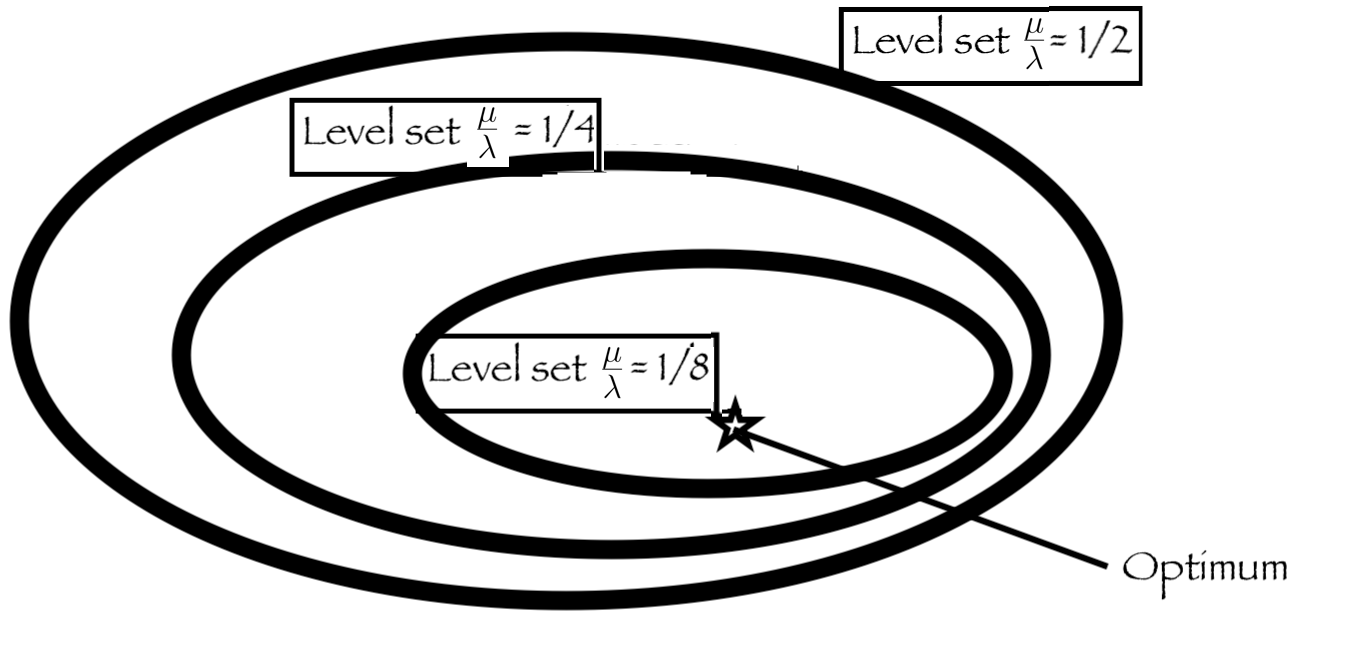
\includegraphics[width=.4\textwidth]{sections/appendix/foga2021-kbest/samples/joli.png}
	\caption{\label{zoli}Assume that we consider a fixed ratio $\mu/\lambda$ and that $\lambda$ goes to $\infty$. The average of selected points, in an unweighted setting and with uniform sampling, converges to the center of the area corresponding to the ratio $\mu/\lambda$: we will not converge to the optimum if that optimum is not the middle of the sublevel. This explains why we need $\mu/\lambda\to 0$ as $\lambda \to \infty$: we do not want to stay at a fixed sublevel. }
	\label{fig:levelset}
\end{figure}
\begin{rmq}[Comparison with random search] The asymptotic
rate obtained for the $\mu$-best averaging approach is of order $\lambda^{-\frac{2(\alpha-1)}{d+2(\alpha-2)}}$,
which is strictly better than the $\lambda^{-2/d}$ rate obtained
with random search, as soon as $d>2$ (because $\alpha>2$) .
This theorem then proves our claim on a wide range of functions. 
\end{rmq}
% \begin{rmq}[Non-smooth or high-dimensional functions]
% Moreover,
% thanks to Lemma~\ref{lem:sandwich}, both rates hold also for the
% expectation of the quadratic distance to the optimum $x^{\star}$: interestingly, this result becomes true for any $\tilde f = g \circ f$ for $g$ increasing and $f$ verifying Assumption \ref{ass:principal}. This extension, classical in evolutionary computation, is valid for our setting (see Section \ref{invar}).
% Results based on surrogate models (e.g. \cite{bach}) are not applicable here. Even in the differentiable case, our results is faster when the ratio smoothness/dimension is small.
% \end{rmq}


% \begin{rmq}
% The results we show are asymptotic in $\lambda$, and do not quantify the domain of validity of the bounds, hence the number of samples $\lambda$ might be exponential in function of the dimension for the bound to be valid non asymptotically. 
% \end{rmq}

\begin{rmq}[Comparison with~\cite{ppsnkbest}] ~\cite{ppsnkbest} obtained a rate of order $\lambda^{-1}$ for the sphere function. This rate is better than the one described in Theorem~\ref{thm:principal}. This comes from the bias term in Lemma~\ref{lem:condit-upper}. Indeed for the sphere function, sublevel sets are symmetric, hence the bias term equals $0$, which is not the case in general for functions satisfying Assumption~\ref{ass:principal}. In this paper we are able to deal with potentially non symmetric functions. One can remark, that if the sublevel sets are symmetric the bias term vanishes and we recover the rate of~\cite{ppsnkbest}.
\end{rmq}
% \begin{proof}
% In what follows, we will use many times a decomposition of the form
% \[
% h(Y)=h(Y)\bigg[\mathbb{I}_{g(Y)\le a}+\mathbb{I}_{g(Y)>a}\bigg]
% \]
% All the $h(Y)\mathbb{I}_{g(Y)>a}$ will be treated using the Hoeffding
% inequality and the fact that $f$ is bounded in essentially the same
% way. As such, we leave this for the end of the proof and we focus
% on the $\mathbb{I}_{g(Y)\leq a}$ term. \\
% We first decompose 
% \[
% f\left(\bar{X}_{(\mu)}\right)=f\left(\bar{X}_{(\mu)}\right)\left[\mathbb{I}_{f\left(X_{(\mu+1)}\right)\leq h_{0}}+\mathbb{I}_{f\left(X_{(\mu+1)}\right)>h_{0}}\right]
% \]
% where $h_{0}>0$ is sufficiently small so that for $h\leq h_{0}$,
% the conclusion of lemma~\ref{lem:condit-upper} holds. We first concentrate
% on the expectation of the first term. We use the notation $\mathbb{J}=\mathbb{I}_{f\left(X_{(\mu+1)}\right)\leq h_{0}}$.
% Note that this is a random variable generated by $f(X_{(\mu+1)})$.
% By lemma~\ref{lem:condit-upper}, we have 
% \begin{align*}
% \mathbb{E}_{X_{1},...X_{\lambda}\sim U(B(0,r))} & \left[f\left(\bar{X}_{(\mu)}\right)\mathbb{I}_{f\left(X_{(\mu+1)}\right)\leq h_{0}}\right]\\
%  & =\mathbb{E}\left[\mathbb{E}\left[f\left(\bar{X}_{(\mu)}\right)\mathbb{I}_{f\left(X_{(\mu+1)}\right)\leq h_{0}}|f\left(X_{(\mu+1)}\right)\right]\right]\\
%  & \leq\mathbb{E}\left[\mathbb{I}_{f\left(X_{(\mu+1)}\right)\leq h_{0}}[C\frac{f(X_{(\mu+1)})}{\mu}+O(f(X_{(\mu+1)})^{\alpha-1})]\right]\\
%  & \leq C'\mathbb{E}\left[\frac{f(X_{(\mu+1)})}{\mu}+f(X_{(\mu+1)})^{\alpha-1}\right]
% \end{align*}
% for some constant $C'>0$. For the first term above, we do another
% decomposition to use lemma 4
% \[
% f(X_{(\mu+1)})=f(X_{(\mu+1)})\bigg\{\mathbb{I}{}_{f\left(X_{(\mu+1)}\right)\leq L(r-||x^{\star}||)^{2}}+\mathbb{I}{}_{f\left(X_{(k+1)}\right)>L(r-||x^{\star}||)^{2}}\bigg\}
% \]
% As previously, we leave aside for now the second term. By lemma 4
% and then lemma 3 and using a Stirling approximation for the ratio
% of $\Gamma$ factors, we obtain
% \begin{align*}
% \mathbb{E}\left[f(X_{(\mu+1)})\mathbb{I}{}_{f\left(X_{(\mu+1)}\right)\leq L(r-||x^{\star}||)^{2}}\right] & \le C_{2}^{-1}\mu^{2/d}\mathbb{E}\left[f(X_{(1)})-f(x^{\star})\right]\\
%  & \le C_{1}C_{2}^{-1}\mu^{2/d}\bigg[\lambda^{-\frac{2}{d}}+o(\lambda^{-\frac{2}{d}})\bigg]
% \end{align*}
% We now study the term $f(X_{(\mu+1)})^{\alpha-1}$. We decompose again
% and focus on $\mathbb{E}f(X_{(\mu+1)})^{\alpha-1}\mathbb{I}{}_{f\left(X_{(\mu+1)}\right)\leq L(r-||x^{\star}||)^{2}}$.
% By lemma 4, we get
% \[
% \mathbb{E}f(X_{(\mu+1)})^{\alpha-1}\mathbb{I}{}_{f\left(X_{(\mu+1)}\right)\leq L(r-||x^{\star}||)^{2}}\le\mu^{2/d}C_{2}^{-1}\mathbb{E}\biggg[\mathbb{E}_{X_{1},...X_{\lambda}\sim }\left[f(X_{(1)})|f(X_{(\mu+1)})=h\right]\biggg]^{\alpha-1}
% \]
% We now use Jensen's inequality (for conditional expectation) on the
% convex function $u\mapsto u^{\alpha-1}$ to get
% \[
% \mathbb{E}f(X_{(\mu+1)})^{\alpha-1}\mathbb{I}{}_{f\left(X_{(k+1)}\right)\leq L(r-||x^{\star}||)^{2}}\le\mu^{\alpha/d}C_{2}^{-(\alpha-1)}\mathbb{E}_{X_{1,\cdots,}X_{\lambda}\sim U(B(0,r))}[f(X_{(1)})^{\alpha-1}]
% \]
% We compute the last quantity. By a proof similar to the one in lemma
% 3, we obtain, with $u_{\alpha}=\left(L\left(r-||x^{\star}||\right)^{2\alpha-2}-L\left(r+||x^{\star}||\right)^{2\alpha-2}\right)$
% \[
% \mathbb{E}_{X_{1},...X_{\lambda}\sim U(B(0,r)) }\left[ f(X_{(1)})^{\alpha-1}\right]=(\alpha-1)Lr^{2}\frac{2}{d}\frac{\Gamma(\frac{2}{d}(\alpha-1))\Gamma(\lambda+1)}{\Gamma(\lambda+1+2(\alpha-1)/d)}+u_{\alpha}\mathbb{P}_{X\sim U(B(0,r))}\left[||X-x^{\star}||\geq r-||x^{\star}||\right]^{\lambda}
% \]
% It remains to bound 
% \[
% \mathbb{E}_{X_{1},...X_{\lambda}\sim U(B(0,r))}\left[f\left(\bar{X}_{(\mu)}\right)\mathbb{I}_{f\left(X_{(\mu+1)}\right)>h_{0}}\right]
% \]
% \[
% \mathbb{E}\left[f(X_{(\mu+1)})\mathbb{I}{}_{f\left(X_{(\mu+1)}\right)>L(r-||x^{\star}||)^{2}}\right]
% \]
% \[
% \mathbb{E}f(X_{(\mu+1)})^{\alpha-1}\mathbb{I}{}_{f\left(X_{(\mu+1)}\right)>L(r-||x^{\star}||)^{2}}
% \]
% Recall that $f$ is upper-bounded (for instance because it is continuous
% on a compact set). Each quantity above can then be upper-bounded by
% a constant times $\mathbb{P}(f(X_{(\mu+1)})>a)$ for some $a>0$.
% We now note that 
% \[
% \mathbb{P}_{X_{1},\cdots,X_{\lambda}\sim U(B(0,r))}\left(f(X_{(\mu+1)})>a\right)=\mathbb{P}_{U\sim B(n,(a/r)^{d})}(U\le\mu)
% \]
% where $\mathcal{B}(n,p)$ means a binomial variable of parameters
% $(n,p)$ for some $a>0$. Let now $\delta=\lambda(\frac{a}{r})^{d}-\mu$.
% Assume that $\delta>0$. Then Hoeffding's inequality gives
% \[
% \mathbb{P}_{U\sim\mathcal{B}(n,(a/r)^{d})}(U\le\mu)\le\exp(-\frac{2\delta^{2}}{\lambda})
% \]
% By taking $b=\min a_{i}$ for the $a_{i}=a$ appearing above, and
% corresponding $\delta$ we thus obtain Note that theHence we obtain
% \[
% \mathbb{E}_{X_{1},...X_{\lambda}\sim U(B(0,r))}\left[f\left(\bar{X}_{(\mu)}\right)\right]\le C(\mu^{\alpha/d}\lambda^{\alpha/d}+\mu^{2/d-1}\lambda^{-2/d}+\mu^{2/d-1}o(\lambda^{-2/d})+\exp(-\frac{2\delta^{2}}{\lambda}))
% \]
% \end{proof}
